\documentclass[11pt,a4paper]{article}
\usepackage[utf8]{inputenc}
\usepackage{graphicx}
\usepackage{geometry}
\usepackage{tikz}
\usepackage{xcolor}
\usepackage{enumitem}
\usepackage{fancyhdr}
\usepackage{multicol}
\usepackage{float}

% Page setup for poster with 4:10 aspect ratio
\geometry{
  paperwidth=400mm,  % 4 units wide
  paperheight=1000mm, % 10 units high (4:10 ratio)
  margin=15mm
}

% Define colors
\definecolor{lightblue}{RGB}{173,216,230}
\definecolor{darkblue}{RGB}{0,51,102}
\definecolor{gold}{RGB}{255,215,0}
\definecolor{green}{RGB}{34,139,34}
\definecolor{red}{RGB}{220,20,60}

% Custom commands
\newcommand{\posterbox}[2]{
  \begin{tikzpicture}
    \node[rectangle, draw=darkblue, fill=white, minimum width=0.9\textwidth, minimum height=#1, rounded corners=5pt] {
      \begin{minipage}{0.85\textwidth}
        #2
      \end{minipage}
    };
  \end{tikzpicture}
}

\newcommand{\headerbox}[2]{
  \begin{tikzpicture}
    \node[rectangle, draw=darkblue, fill=darkblue, minimum width=0.9\textwidth, minimum height=#1, rounded corners=5pt] {
      \begin{minipage}{0.85\textwidth}
        \textcolor{white}{\Large\textbf{#2}}
      \end{minipage}
    };
  \end{tikzpicture}
}

\begin{document}

% Header
\begin{center}
  
\begin{tikzpicture}
    \node[rectangle, fill=darkblue, minimum width=\textwidth, minimum height=2.5cm, rounded corners=10pt] {
      \begin{minipage}{0.9\textwidth}
        \centering
        \textcolor{white}{\Huge\textbf{Antique Bidderly}} \\[0.3cm]
        \textcolor{white}{\Large\textbf{Milan Tamang}} \\
        \textcolor{white}{\normalsize BSc (Hons) in Software Engineering - UC3F1410SE}
      \end{minipage}
    };
  \end{tikzpicture}
\end{center}

\vspace{0.5cm}

% Main content in 2 columns for taller format
\begin{multicols}{2}

% Introduction
\headerbox{1.5cm}{Introduction}
\vspace{0.1cm}
\posterbox{7cm}{
Antique Bidderly is a modern, real-time auction platform built with the MERN stack (MongoDB, Express.js, React, Node.js) that revolutionizes the antique trading experience. The system leverages WebSocket technology for live bidding, integrated payment processing, and comprehensive admin management to create a seamless auction environment for antique enthusiasts and collectors.

The platform addresses the limitations of traditional auction systems by providing a comprehensive digital solution that combines modern web technologies with user-friendly interfaces and robust backend infrastructure.
}

\vspace{0.5cm}

% Problem Statement
\headerbox{1.5cm}{Problem Statement}
\vspace{0.1cm}
\posterbox{7cm}{
Traditional antique auctions face several challenges:
\begin{itemize}[leftmargin=*]
\item Limited accessibility due to geographical constraints
\item Lack of real-time bidding capabilities
\item Inefficient payment processing systems
\item Poor user experience with outdated interfaces
\item Difficulty in managing auction approvals and monitoring
\item No automated notification systems for bidders
\item High operational costs for physical auction houses
\item Limited market reach for sellers and buyers
\end{itemize}
}

\vspace{0.5cm}

% Purpose
\headerbox{1.5cm}{Purpose}
\vspace{0.1cm}
\posterbox{7cm}{
The primary objectives of Antique Bidderly include:
\begin{itemize}[leftmargin=*]
\item Provide a modern, accessible online auction platform
\item Enable real-time bidding with WebSocket technology
\item Integrate secure payment processing (eSewa)
\item Implement comprehensive admin approval system
\item Create responsive, user-friendly interfaces
\item Automate notification systems for users
\item Ensure secure authentication and authorization
\item Facilitate global market access for antique trading
\end{itemize}
}

\vspace{0.5cm}

% Implementation
\headerbox{1.5cm}{Implementation}
\vspace{0.1cm}
\posterbox{7cm}{
\textbf{Frontend Technologies:}
\begin{itemize}[leftmargin=*]
\item React.js with TypeScript for type-safe development
\item Tailwind CSS for modern, responsive styling
\item Socket.IO client for real-time communication
\item Vite build tool for fast development and optimized builds
\item React Router for seamless navigation
\end{itemize}

\textbf{Backend Technologies:}
\begin{itemize}[leftmargin=*]
\item Node.js with Express.js framework
\item PostgreSQL database for reliable data storage
\item Socket.IO server for real-time bidirectional communication
\item JWT authentication for secure user sessions
\item Multer middleware for file upload handling
\end{itemize}

\textbf{Payment Integration:}
\begin{itemize}[leftmargin=*]
\item eSewa payment gateway integration
\item Secure transaction processing and verification
\item Comprehensive order management system
\end{itemize}
}

\vspace{0.5cm}

% How it works
\headerbox{1.5cm}{How it works}
\vspace{0.1cm}
\posterbox{7cm}{
\begin{center}
\textbf{User Registration + Authentication + Real-time Bidding + Payment Processing}
\end{center}

The system operates through a seamless workflow:
\begin{enumerate}[leftmargin=*]
\item Users register and authenticate securely
\item Sellers create auctions with detailed descriptions
\item Admin approves auctions for bidding
\item Real-time bidding occurs via WebSocket connections
\item Automated notifications keep users informed
\item Secure payment processing completes transactions
\item Order management and delivery coordination
\item Post-auction feedback and rating system
\end{enumerate}
}

\vspace{0.5cm}

% Technical Stack
\headerbox{1.5cm}{Technical Stack}
\vspace{0.1cm}
\posterbox{7cm}{
\textbf{Frontend Technologies:}
\begin{itemize}[leftmargin=*]
\item React.js with TypeScript
\item Tailwind CSS for styling
\item Socket.IO client
\item Vite build tool
\item React Router for navigation
\end{itemize}

\textbf{Backend Technologies:}
\begin{itemize}[leftmargin=*]
\item Node.js with Express.js
\item PostgreSQL database
\item Socket.IO server
\item JWT authentication
\item Multer for file uploads
\end{itemize}

\textbf{Payment Integration:}
\begin{itemize}[leftmargin=*]
\item eSewa payment gateway
\item Secure transaction processing
\item Order management system
\end{itemize}
}

\vspace{0.5cm}

% Key Features
\headerbox{1.5cm}{Key Features}
\vspace{0.1cm}
\posterbox{7cm}{
\begin{itemize}[leftmargin=*]
\item Real-time live bidding with WebSocket technology
\item User authentication and authorization system
\item Auction creation and management tools
\item Admin approval system for quality control
\item Payment processing integration with eSewa
\item Automated notification system for users
\item Responsive design for all devices
\item File upload for auction images and documents
\item Category management for organized browsing
\item Bid history tracking and analytics
\item Order management and fulfillment
\item User profiles and personalized dashboards
\item Real-time chat and communication features
\end{itemize}
}

\vspace{0.5cm}

% Conclusion
\headerbox{1.5cm}{Conclusion}
\vspace{0.1cm}
\posterbox{7cm}{
Antique Bidderly successfully demonstrates the effectiveness of modern web technologies in creating a comprehensive auction platform. The system provides:

\begin{itemize}[leftmargin=*]
\item Seamless real-time bidding experience
\item Secure payment integration
\item Comprehensive admin management
\item Responsive user interfaces
\item Automated notification systems
\end{itemize}

\textbf{Future Plans:} Deploy to production, implement advanced analytics, add mobile applications, and expand payment gateway options. The platform is designed to scale and adapt to growing market demands while maintaining security and user experience standards.
}

\end{multicols}

\vspace{1cm}

% Bottom section
\begin{center}
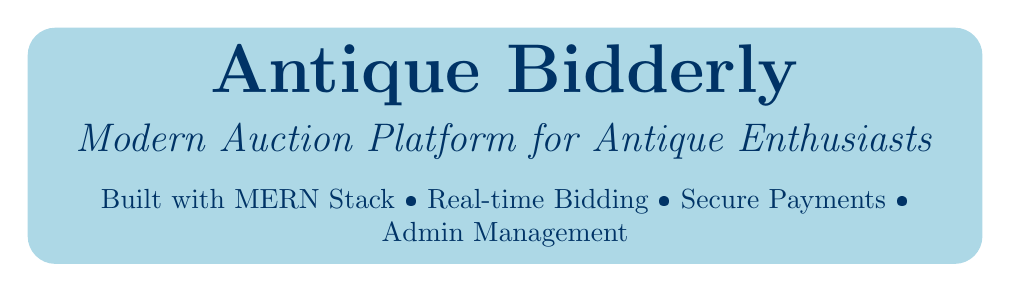
\begin{tikzpicture}
\node[rectangle, fill=lightblue, minimum width=\textwidth, minimum height=3cm, rounded corners=10pt] {
\begin{minipage}{0.9\textwidth}
\centering
\textcolor{darkblue}{\Huge\textbf{Antique Bidderly}} \\[0.2cm]
\textcolor{darkblue}{\Large\textit{Modern Auction Platform for Antique Enthusiasts}} \\[0.3cm]
\textcolor{darkblue}{\normalsize Built with MERN Stack • Real-time Bidding • Secure Payments • Admin Management}
\end{minipage}
};
\end{tikzpicture}
\end{center}

\end{document}
